% unit: u21
% sources: sources/083-determinant-formulas-and-cofactors.txt, sources/037-lecture-19-determinant-formulas-and-cofactors.txt, sources/188-mit18-06scf11-ses2-6sum-pdf-download-file.txt, sources/038-problem-solving-determinants.txt, sources/189-mit18-06scf11-ses2-6prob-pdf-download-file.txt, sources/190-mit18-06scf11-ses2-6sol-pdf-download-file.txt
\section{Determinant formulas and cofactors}\label{sec:u21}

Section~\ref{sec:u20} defined the determinant by three properties and computed it by
elimination: $\det A$ is $\pm$ the product of the pivots. This section derives two explicit
formulas from the same properties. The \emph{big formula} writes $\det A$ as a sum of $n!$
signed products, one entry from each row and each column. The \emph{cofactor formula} groups
those products to express an $n\times n$ determinant through determinants of size $n-1$. We
finish with a family of tridiagonal matrices whose determinants repeat with period six.

\subsection{Splitting the rows: from \texorpdfstring{$2\times 2$}{2 by 2} to the big formula}

Linearity in each row (property 3) lets us split a row into pieces. For a $2\times 2$ matrix
split row~1 as $(a,b)=(a,0)+(0,b)$, then split row~2 in each piece:
\[
  \begin{vmatrix}a&b\\c&d\end{vmatrix}
  =\begin{vmatrix}a&0\\c&d\end{vmatrix}+\begin{vmatrix}0&b\\c&d\end{vmatrix}
  =\begin{vmatrix}a&0\\c&0\end{vmatrix}+\begin{vmatrix}a&0\\0&d\end{vmatrix}
  +\begin{vmatrix}0&b\\c&0\end{vmatrix}+\begin{vmatrix}0&b\\0&d\end{vmatrix}.
\]
The first and last pieces have a zero column, so they are singular and vanish. The second is
diagonal, $ad$. The third is $bc$ times the determinant of the row exchange
$\left[\begin{smallmatrix}0&1\\1&0\end{smallmatrix}\right]$, which is $-1$. So
$\det A=ad-bc$, now derived rather than remembered.

For a $3\times 3$ matrix the same splitting produces $3\cdot 3\cdot 3=27$ pieces, each with
one entry from each row. A piece survives only if its three entries also lie in three
\emph{different columns}; otherwise it has a zero column. The survivors are the six patterns of
Figure~\ref{fig:u21-survivors}, and each equals the product of its entries times the
determinant of a permutation matrix:
\[
  \det A=a_{11}a_{22}a_{33}-a_{11}a_{23}a_{32}-a_{12}a_{21}a_{33}+a_{12}a_{23}a_{31}
  +a_{13}a_{21}a_{32}-a_{13}a_{22}a_{31}.
\]
For example the term $a_{12}a_{23}a_{31}$ uses columns $(2,3,1)$; two exchanges (rows 1 and
3, then rows 2 and 3) restore the order $(1,2,3)$, so its sign is $+$.

\begin{figure}[ht]
  \centering
  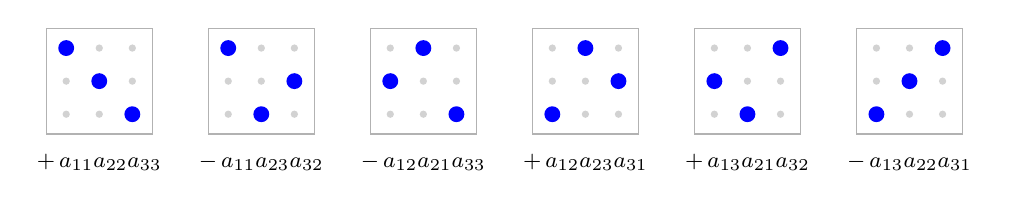
\begin{tikzpicture}[scale=0.42,font=\footnotesize]
    \foreach \a/\b/\c/\sg [count=\k from 0] in {1/2/3/+, 1/3/2/-, 2/1/3/-, 2/3/1/+, 3/1/2/+, 3/2/1/-}{
      \begin{scope}[shift={(\k*4.9,0)}]
        \draw[gray!60] (0.4,0.4) rectangle (3.6,3.6);
        \foreach \i in {1,2,3} {\foreach \j in {1,2,3} {\fill[gray!35] (\j,4-\i) circle (0.11);}}
        \fill[blue] (\a,3) circle (0.24);
        \fill[blue] (\b,2) circle (0.24);
        \fill[blue] (\c,1) circle (0.24);
        \node at (2,-0.45) {$\sg\,a_{1\a}a_{2\b}a_{3\c}$};
      \end{scope}}
  \end{tikzpicture}
  \caption{The six nonzero pieces of a $3\times 3$ determinant: one entry from each row and
  each column, i.e.\ the positions of the $1$'s in a permutation matrix. The sign is the
  determinant of that permutation matrix: $+$ for an even number of row exchanges, $-$ for an
  odd number.}
  \label{fig:u21-survivors}
\end{figure}

\begin{definition}[Sign of a permutation]\label{def:u21-sign}
A permutation $\sigma$ of $\{1,\dots,n\}$ corresponds to the permutation matrix $P_\sigma$
whose row $i$ has its $1$ in column $\sigma(i)$. Its \emph{sign} is
$\operatorname{sgn}\sigma=\det P_\sigma$, which is $+1$ if $P_\sigma$ is reached from $I$ by
an even number of row exchanges and $-1$ if by an odd number.
\end{definition}

\begin{theorem}[The big formula]\label{thm:u21-big}
For an $n\times n$ matrix $A$,
\[
  \det A=\sum_{\sigma}\operatorname{sgn}(\sigma)\,a_{1\sigma(1)}a_{2\sigma(2)}\cdots a_{n\sigma(n)},
\]
the sum running over all $n!$ permutations $\sigma=(\alpha,\beta,\dots,\omega)$ of the column
numbers.
\end{theorem}

\begin{proof}
Write row $i$ of $A$ as $\sum_j a_{ij}\vb{e}_j\T$, where $\vb{e}_j\T$ is row $j$ of $I$. Using
linearity in row~1, then in row~2, and so on, $\det A$ becomes a sum over all choices of
column numbers $(j_1,\dots,j_n)$:
\[
  \det A=\sum_{j_1,\dots,j_n}a_{1j_1}a_{2j_2}\cdots a_{nj_n}\,
  \det\begin{bmatrix}\vb{e}_{j_1}\T\\ \vdots\\ \vb{e}_{j_n}\T\end{bmatrix}.
\]
If two of the $j$'s coincide, the last matrix has two equal rows and its determinant is $0$.
Otherwise $(j_1,\dots,j_n)$ is a permutation $\sigma$ and the matrix is $P_\sigma$, whose
determinant is $\operatorname{sgn}\sigma$.
\end{proof}

Why $n!$ terms: the entry from row~1 can be chosen in $n$ columns, the entry from row~2 in the
$n-1$ columns still unused, and so on: $2$ terms for $n=2$, $6$ for $n=3$, $24$ for $n=4$.
Half have each sign (for $n\ge 2$). The formula reproduces the properties; for instance
$\det I=1$ because only the identity permutation picks no zero entry of $I$. Conversely, the
formula \emph{defines} a function with properties 1--3, which settles the loose end of
Section~\ref{sec:u20}: the determinant exists, so a permutation cannot be both even and odd.

\begin{trap}
The ``down-right diagonals are $+$, down-left diagonals are $-$'' picture of the $3\times 3$
formula does not extend to $4\times 4$. The $4\times 4$ anti-diagonal permutation $(4,3,2,1)$
needs two exchanges (rows 1 and 4, rows 2 and 3), so its term carries a $+$ sign. Always count
exchanges, or use cofactors.
\end{trap}

\begin{example}[Most terms vanish]\label{ex:u21-sparse}
For
\[
  A=\begin{bmatrix}0&0&1&1\\0&1&1&0\\1&1&0&0\\1&0&0&1\end{bmatrix}
\]
look for ways to pick a nonzero entry in every row and column. Row~1 can use column~3 or
column~4, and each choice forces the rest. If row~1 uses column~4, row~4 must use column~1,
then row~3 column~2 and row~2 column~3: the permutation $(4,3,2,1)$, sign $+$, contributing
$+1$. If row~1 uses column~3, row~2 must use column~2, row~3 column~1 and row~4 column~4:
the permutation $(3,2,1,4)$, which one exchange (rows 1 and 3 of its permutation matrix) puts
in order, so its sign is $-$ and it contributes $-1$.
Row~1 has no other nonzero entries, so these are the only two of the $24$ terms, and
$\det A=1-1=0$. The matrix must be singular, and indeed
row~1 $-$ row~2 $+$ row~3 $-$ row~4 $=\vb{0}$.
\end{example}

\subsection{Cofactors}

Collect the terms of the big formula that contain a particular entry $a_{1j}$. What
multiplies $a_{1j}$ is built from the other rows and the other columns, one entry from each:
it is (up to sign) a determinant of size $n-1$.

\begin{definition}[Minor and cofactor]\label{def:u21-cofactor}
The \emph{minor} $M_{ij}$ is the $(n-1)\times(n-1)$ matrix obtained from $A$ by deleting row
$i$ and column $j$. The \emph{cofactor} of $a_{ij}$ is
\[
  C_{ij}=(-1)^{i+j}\det M_{ij}.
\]
The signs $(-1)^{i+j}$ form a checkerboard starting with $+$ in the top-left corner.
\end{definition}

\begin{theorem}[Cofactor expansion]\label{thm:u21-cofactor}
For each row $i$,
\[
  \det A=a_{i1}C_{i1}+a_{i2}C_{i2}+\cdots+a_{in}C_{in},
\]
and likewise down each column $j$: $\det A=a_{1j}C_{1j}+\cdots+a_{nj}C_{nj}$.
\end{theorem}

\begin{proof}
\emph{Row 1.} By linearity in row~1, $\det A=\sum_j a_{1j}\det A_j$, where $A_j$ is $A$ with
row~1 replaced by $\vb{e}_j\T$. In $A_j$ subtract multiples of row~1 from the other rows to
clear column $j$ below the $1$ (property 5, no change). Then move column $j$ to the front by
$j-1$ exchanges of neighbouring columns; each reverses the sign (exchanging columns is allowed
because $\det A\T=\det A$), and the other columns keep their order. The result is the block matrix
\[
  \begin{bmatrix}1&\vb{0}\T\\ \vb{0}&M_{1j}\end{bmatrix}.
\]
Its determinant is $\det M_{1j}$, because as a function of the $(n-1)\times(n-1)$ matrix $M$,
the determinant of $\left[\begin{smallmatrix}1&\vb{0}\T\\ \vb{0}&M\end{smallmatrix}\right]$
satisfies the three defining properties, so it equals $\det M$ by uniqueness
(Section~\ref{sec:u20}). Hence $\det A_j=(-1)^{j-1}\det M_{1j}=C_{1j}$.

\emph{Row $i$.} Move row $i$ to the top by $i-1$ exchanges of neighbouring rows, keeping the
other rows in order. The determinant gains the factor $(-1)^{i-1}$, the new first row is row
$i$ of $A$, and its minors are the $M_{ij}$. So
$\det A=(-1)^{i-1}\sum_j a_{ij}(-1)^{1+j}\det M_{ij}=\sum_j a_{ij}C_{ij}$.

\emph{Columns.} Apply the row expansion to $A\T$.
\end{proof}

For a $2\times 2$ matrix the cofactors along row~1 are $C_{11}=d$ and $C_{12}=-c$, giving
$ad+b(-c)$. For $3\times 3$ the expansion along row~1 is
\[
  \det A=a_{11}(a_{22}a_{33}-a_{23}a_{32})+a_{12}(-a_{21}a_{33}+a_{23}a_{31})+a_{13}(a_{21}a_{32}-a_{22}a_{31}),
\]
which is the six-term formula regrouped; the middle parenthesis carries the minus sign of the
$(1,2)$ position.

\begin{example}[Expanding along a convenient row]\label{ex:u21-expand}
Take the matrix of Section~\ref{sec:u20} whose pivots $2,-8,1$ gave $\det A=-16$:
\[
  A=\begin{bmatrix}2&1&1\\4&-6&0\\-2&7&2\end{bmatrix}.
\]
Along row~1:
\[
  C_{11}=+\begin{vmatrix}-6&0\\7&2\end{vmatrix}=-12,\quad
  C_{12}=-\begin{vmatrix}4&0\\-2&2\end{vmatrix}=-8,\quad
  C_{13}=+\begin{vmatrix}4&-6\\-2&7\end{vmatrix}=16,
\]
so $\det A=2(-12)+1(-8)+1(16)=-16$. Row~2 contains a zero, which saves one minor: with
$C_{21}=-\left|\begin{smallmatrix}1&1\\7&2\end{smallmatrix}\right|=5$ and
$C_{22}=+\left|\begin{smallmatrix}2&1\\-2&2\end{smallmatrix}\right|=6$,
$\det A=4\cdot 5+(-6)\cdot 6+0\cdot C_{23}=-16$ again.
\end{example}

There are now three ways to compute a determinant, and each has its use.
\begin{center}
\begin{tabular}{@{}lll@{}}
  \toprule
  Method & Work for $n\times n$ & Best when \\
  \midrule
  Pivots (elimination) & about $n^3/3$ operations & any numerical matrix \\
  Big formula & $n!$ products of $n$ entries & very few nonzero entries \\
  Cofactors & reduces size $n$ to size $n-1$ & a row or column with many zeros; patterns \\
  \bottomrule
\end{tabular}
\end{center}
The pivots have all the complexity built in efficiently; the big formula spreads it out
completely; cofactors sit in between and are the tool for proving recursions.

\subsection{Tridiagonal matrices of ones}

Let $A_n$ be the $n\times n$ matrix with $1$'s on the main diagonal and the two diagonals
next to it, and $0$ elsewhere:
\[
  A_1=\begin{bmatrix}1\end{bmatrix},\quad
  A_2=\begin{bmatrix}1&1\\1&1\end{bmatrix},\quad
  A_3=\begin{bmatrix}1&1&0\\1&1&1\\0&1&1\end{bmatrix},\quad
  A_4=\begin{bmatrix}1&1&0&0\\1&1&1&0\\0&1&1&1\\0&0&1&1\end{bmatrix}.
\]
Directly, $|A_1|=1$ and $|A_2|=0$. For $A_3$ the big formula has only three nonzero terms:
$a_{11}a_{22}a_{33}=1$, $-a_{11}a_{23}a_{32}=-1$ and $-a_{12}a_{21}a_{33}=-1$, so $|A_3|=-1$.

\begin{theorem}[A three-term recursion]\label{thm:u21-tridiag}
For $n\ge 3$, $\ |A_n|=|A_{n-1}|-|A_{n-2}|$. Consequently the sequence $|A_n|$ is
\[
  1,\ 0,\ -1,\ -1,\ 0,\ 1,\ \ 1,\ 0,\ -1,\ -1,\ 0,\ 1,\ \dots
\]
and repeats with period $6$.
\end{theorem}

\begin{proof}
Expand along row~1, whose only nonzero entries are $a_{11}=a_{12}=1$. The cofactor $C_{11}$
is the determinant of the lower-right block, which is $A_{n-1}$. The cofactor $C_{12}$ is
$-\det M_{12}$, where $M_{12}$ (rows $2,\dots,n$ and columns $1,3,\dots,n$) has first column
$(1,0,\dots,0)$. Expanding $M_{12}$ down that column leaves its lower-right block, which is
$A_{n-2}$. Hence $|A_n|=|A_{n-1}|-|A_{n-2}|$. Applying the recursion twice,
$|A_{n+3}|=|A_{n+2}|-|A_{n+1}|=(|A_{n+1}|-|A_n|)-|A_{n+1}|=-|A_n|$, so
$|A_{n+6}|=|A_n|$. Starting from $1,0$ the recursion gives $-1,-1,0,1$ and then repeats.
\end{proof}

So $|A_4|=|A_3|-|A_2|=-1$, and for instance $|A_{61}|=|A_1|=1$, a value no one would guess by
looking at a $61\times 61$ matrix. Figure~\ref{fig:u21-period} plots the pattern.

\begin{figure}[ht]
  \centering
  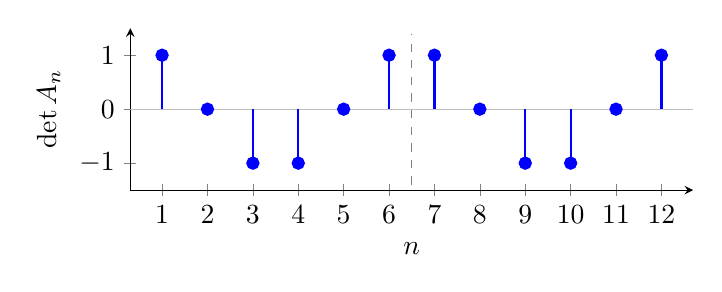
\begin{tikzpicture}
    \begin{axis}[width=0.72\textwidth,height=0.3\textwidth,xmin=0.3,xmax=12.7,ymin=-1.5,ymax=1.5,
        xtick={1,...,12},ytick={-1,0,1},xlabel={$n$},ylabel={$\det A_n$},axis lines=left]
      \draw[gray!50] (axis cs:0.3,0) -- (axis cs:12.7,0);
      \draw[dashed,gray] (axis cs:6.5,-1.4) -- (axis cs:6.5,1.4);
      \addplot[ycomb,blue,thick,mark=*,mark options={fill=blue}] coordinates
        {(1,1) (2,0) (3,-1) (4,-1) (5,0) (6,1) (7,1) (8,0) (9,-1) (10,-1) (11,0) (12,1)};
    \end{axis}
  \end{tikzpicture}
  \caption{Determinants of the tridiagonal matrices of ones. The recursion
  $|A_n|=|A_{n-1}|-|A_{n-2}|$ from the cofactor expansion forces period $6$ (dashed line: one
  period).}
  \label{fig:u21-period}
\end{figure}

\subsection{Exercises}

\begin{exercise}\label{ex:u21-cycle}
Compute the determinant of
\[
  A=\begin{bmatrix}0&0&0&1\\1&0&0&0\\0&1&0&0\\0&0&1&0\end{bmatrix}.
\]
Which method do you prefer here, and why?
\end{exercise}

\begin{solution}
The big formula has a single nonzero term, from the permutation $(4,1,2,3)$, with product
$1$. Moving row~1 to the bottom takes three exchanges (rows 1--2, 2--3, 3--4), which turns $A$
into $I$; the permutation is odd, so $\det A=-1$. Cofactors along row~1 give the same with no
searching: the only nonzero entry is $a_{14}=1$, whose minor (rows 2--4, columns 1--3) is $I_3$,
so $\det A=(-1)^{1+4}\cdot 1=-1$. With a single $1$ in each row, either method beats
elimination.
\end{solution}

\begin{exercise}\label{ex:u21-pascal}
The symmetric Pascal matrices have determinant $1$; for instance
$\det\left[\begin{smallmatrix}1&1&1&1\\1&2&3&4\\1&3&6&10\\1&4&10&20\end{smallmatrix}\right]=1$.
Explain why subtracting $1$ from the $(n,n)$ entry (here $20\to 19$) makes the determinant
$0$.
\end{exercise}

\begin{solution}
By linearity in the last row, the new determinant is the old one plus the determinant of the
matrix whose last row is $(0,\dots,0,-1)$. Expanding that matrix along its last row gives
$(-1)\cdot C_{nn}=-\det(\text{Pascal matrix of size }n-1)=-1$, because $(-1)^{n+n}=+1$. So the
determinant drops from $1$ to $1-1=0$. In the example the cofactor is
$\det\left[\begin{smallmatrix}1&1&1\\1&2&3\\1&3&6\end{smallmatrix}\right]=1$.
\end{solution}

\begin{exercise}\label{ex:u21-cyclic5}
Find the determinant of the $5\times 5$ matrix with $x$ on the diagonal, $y$ just to the
right of the diagonal in rows~1--4, $y$ in position $(5,1)$, and zeros elsewhere:
\[
  A=\begin{bmatrix}x&y&0&0&0\\0&x&y&0&0\\0&0&x&y&0\\0&0&0&x&y\\y&0&0&0&x\end{bmatrix}.
\]
\end{exercise}

\begin{solution}
Expand down column~1, which has only $a_{11}=x$ and $a_{51}=y$. Deleting row~1 and column~1
leaves an upper triangular matrix with $x$'s on its diagonal, determinant $x^4$. Deleting
row~5 and column~1 leaves a lower triangular matrix with $y$'s on its diagonal, determinant
$y^4$, and the sign is $(-1)^{5+1}=+1$. Hence $\det A=x\cdot x^4+y\cdot y^4=x^5+y^5$.
\end{solution}

\begin{exercise}\label{ex:u21-allY}
Find the determinant of the $5\times 5$ matrix $B$ with $x$ on the diagonal and $y$ in every
other position.
\end{exercise}

\begin{solution}
Add rows 2--5 to row~1 (property 5, no change): every entry of row~1 becomes $x+4y$. Factor
it out (property 3a), leaving a row of ones. Now subtract $y$ times this row of ones from each of
rows 2--5. Row $k$ had $y$ in every position except $x$ in position $k$, so it becomes $0$
everywhere except $x-y$ in position $k$. The result is upper
triangular with diagonal $1,\,x-y,\,x-y,\,x-y,\,x-y$, so
\[
  \det B=(x+4y)(x-y)^4 .
\]
Check: for $y=0$ this is $x^5=\det(xI)$, and for $x=y$ all rows are equal and the determinant
is $0$.
\end{solution}
